\emph{\gls{Smalltalk}} is the language used in the team, therefore this is the language I used during my internship. To understand the challenges I faced I will briefly present \gls{Smalltalk} and its main characteristics.

\subsection {What is Smalltalk ?}

\emph{\gls{Smalltalk}} is an object-oriented, reflective, dynamically typed programming languages. So let's explain each word:

%@@NO SPACE before :?; in english@@

\begin{itemize}
	\item Object-oriented : in \gls{Smalltalk}, you manipulate objects which send messages (like in Java or C++);
	\item Reflective : each object can inspect or modify its own structure at runtime (like Java, but to a much greater extent);
	\item Dynamically typed : variables don't have a type at compilation, but only when a value is stored in them at runtime;
	\item \textit{Everything is an object}: everything is an object (a class, a message, a method, \dots)
\end{itemize}

\subsection{Smalltalk basics}

\gls{Smalltalk} is based on 2 classes which constitute the conceptual core of this system, \ct{Object} and \ct{Class} (see Figure~\ref{ClassObjectBootStrap}). Here you can see that each element cannot exist alone. The bootstrap is the process which leads to this state. However, since \ct{Class} and \ct{Object} needs other objects such as string, characters, stream, numbers\dots the real bootstrap is more complex.

\begin{figure}[h]
	\centering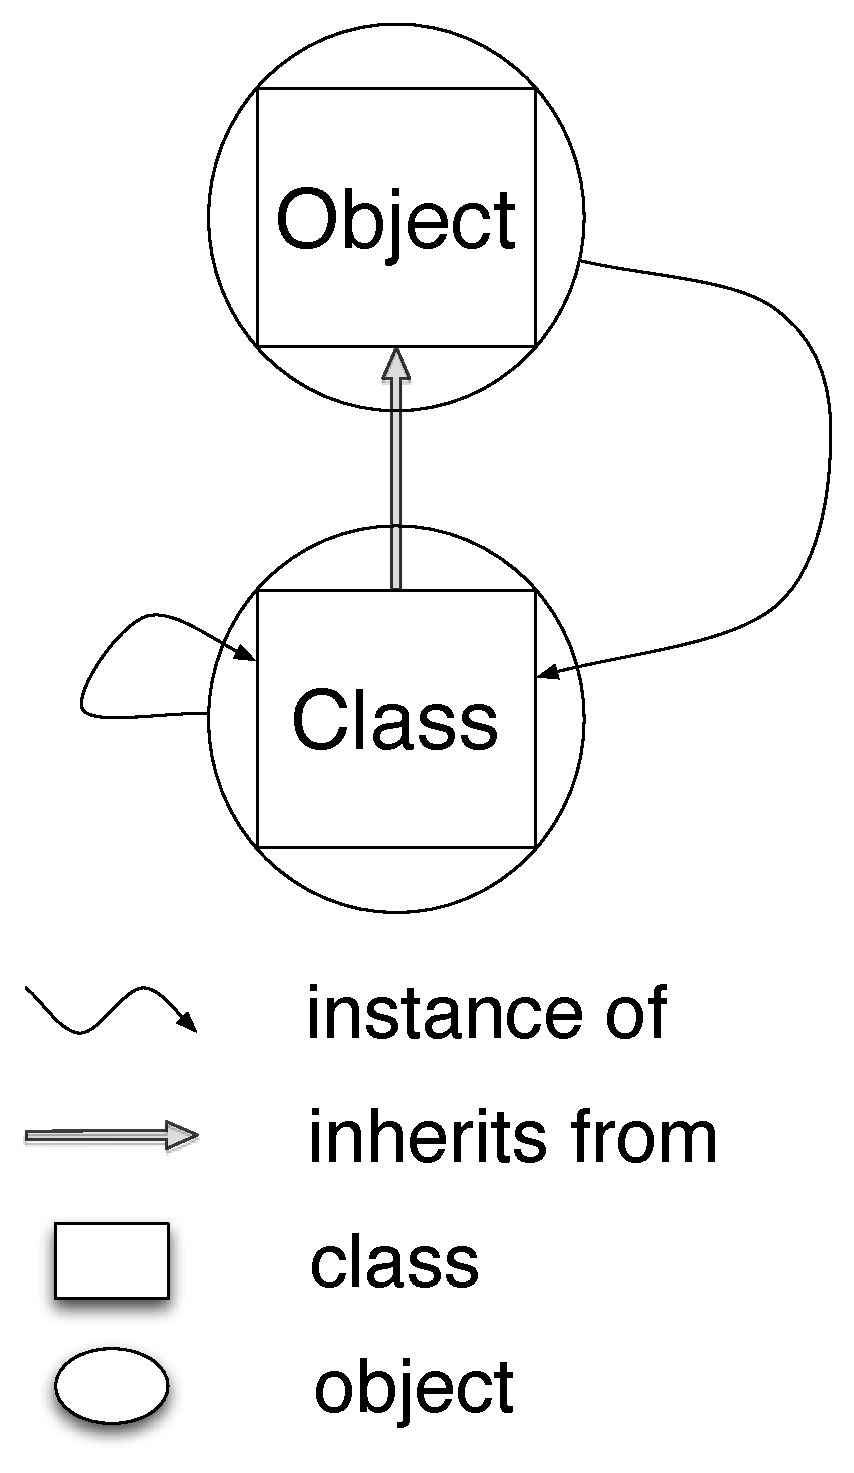
\includegraphics[height = 7cm]{figures/BootStrap}
	\caption{Class and Object bootstrap}
	\label{ClassObjectBootStrap}
\end{figure}
	
The most important thing to know is that a bootstrap is a process where a system is initializing itself via its own execution. It's close to the \emph{Chicken or egg dilemma} where each one deeply depends on the other one (more details will be given in the next chapter, page~\pageref{BootStrap}).

\subsection{Some basics code lines}

Here few examples of \gls{Smalltalk} code to know how to read further examples:

\begin{code}{}
	"Variables declaration"
	| variable1 variable2 |

	"Instance creation"
	variable1 := Point new.
	"Instance setting"
	variable1 x: 1.
	variable1 y: 2.
	
	variable2 := Point new.
	variable2 x: 1.
	variable2 y: 2.
	
	variable1 = variable2. \emph{true}
	variable1 == variable2. \emph{false}
\end{code}
Here, we can see 5 things :
\begin{itemize}
	\item \ct{| |} : it allows you to declare variables.
	\item \ct{:=} : it is the assignment.
	\item \ct{new} : it's a class method which creates a new instance of the receiver, e.g. ``\texttt{Point new}'' sends the message new to the class (which is also an object) Point.
	\item \ct{=} : it tests if two objects represent the same object, it's a \emph{logical} equality. It is a message, asking the receiver (before =) whether it is the same object as the parameter (after the =).
	\item \ct{==} : it tests if two objects point to the same reference, it's a \emph{physical} equality. It is a message also.
\end{itemize}
Let's see a basic method of the \ct{Integer} class:

\begin{code}{}
plus: integer1 andPlus: integer2 

\tab^ self + integer1 + integer2
\end{code}
Here we learn 3 new things:
\begin{itemize}
	\item \ct{:} : the way to specify parameters to most methods.
	\item \ct{self} : the receiver of the method (similar to this in Java).
	\item \ct{\^} : it allows you to return a value\footnotemark. By default a method returns \ct{self}.
\end{itemize}
\footnotetext{You can sometime see $\uparrow$ instead.}
A method is often referred to by the notation \ct{Class$\gg$\#selector} to have an unique notation. So the method we just saw is noted \ct{Integer$\gg$\#plus:andPlus:}. 
One more example to see the last syntax elements, a method of class \ct{Class}:
\begin{code}{}
copyMethodDictionary
	   "This method answer a copy of my method dictionary"
	
	   | result |
	   result := SortedCollection new sort: [:m1 :m2 | m1 selector < m2 selector].
	   self methodDictionary do: [:method |
	       result add: method.
	       Transcript  show: method selector asString, ' added.';cr].
       ^ result
\end{code}
Here we have :
\begin{itemize}
	\item \ct{"some text"} : a comment.
	\item \ct{[:arg | code]} : it's a block (a $\lambda$-expression). They act like anonymous methods where arg is an argument of the block which is used to execute the code. In addition it captures its creation environment - it is a lexical closure.
	\item \ct{rcvr m1; m2} : it's a cascade of messages. It means that the receiver of the second method (m2) is the same that the first method's (m1) receiver, in this case \ct{rcvr}.
\end{itemize}

Now, you know the syntax of \gls{Smalltalk}.

\subsection{The SystemDictionary}

The \emph{System Dictionary} is a dictionary which contains all the global variables, including all the classes of the system. In \gls{Pharo}, the variable \emph{Smalltalk} is, normally, the sole SystemDictionary of the system. We can notice that \emph{Smalltalk} is a global variable, so it contains itself.

\subsection{Special Object Array}

The \gls{Special Objects Array} is basically an array shared between an image and the \gls{VM}. It's an interface allowing the \gls{VM} to know where are special objects it needs.

\paragraph{What is in the Special Objects Array ?}
Here I will give the first ten elements of the \gls{Special Objects Array}:
\begin{itemize}
	\item \ct{nil}\footnote{\ct{nil} is te basic NullPattern object, like \ct{NULL} in C or \ct{null} in Java} 
	\item \ct{true}
	\item \ct{false}
	\item \ct{\#Processor->Processor}
	\item \ct{Bitmap}
	\item \ct{SmallInteger}
	\item \ct{ByteString}
	\item \ct{Array}
	\item \ct{Smalltalk}
	\item \ct{Float}
	\item \dots
\end{itemize}

We can notice that the nineth element is \ct{Smalltalk}, the current SystemDictionary.

\subsection{The Virtual Machine}

As some other languages (especially Java), Smalltalk's methods are converted then interpreted by a \gls{VM}. In fact, the Smalltalk compiler analyzes the code then createss a \ct{CompiledMethod} which is a representation of the method but including more information ready to be executed by a \emph{byteCode} interpreter or JustInTime translator:
\begin{itemize}\label{literal}
	\item the \emph{byteCode} : the source code converted into a language that the \gls{VM} can interpret;
	\item the \emph{literals} : they represent low level objects such as number true, false, strings that are referenced and read by the scanner at compilation time. \emph{Literals} especially store pointers to class referred into the source code.
\end{itemize}

\subsubsection*{Method}
Let's see an example, \ct{String$\gg$\#copy} :

\begin{code}{}
copy

\tab | string |
\tab string := String new: (self size).
\tab self doWithIndex: [:character :index |
\tab \tab string at: index put: character].
\tab ^ string
\end{code}

First, let's explain what this method do :

\begin{itemize}
	\item \ct{| string |} : we declare a new variable named \ct{string}.
	\item \ct{string := String new: (self size)} : it creates a new instance of the class \ct{String} which the size is set at the size of the receiver and then stores it in the variable named \ct{string}.
	\item \ct{self doWithIndex: [:character :index |} : we browse the receiver and for each element, we store the element in the variable \ct{character} end the index of the element in the variable \ct{index}.
	\item \ct{string at: index put: character} : at the index \ct{index} of \ct{string}, we put \ct{character}.
	\item \ct{\^{} string} : we finally return the variable \ct{string}.
\end{itemize}
In a nutshell, this method basically parses the receiver (which is a \ct{String}) and fills up a new \ct{String} with the same value.

\subsubsection*{CompiledMethod}
Now, let's take a look at the corresponding \ct{CompiledMethod}
\begin{itemize}
	\item the \emph{byteCode} : 
	\begin{code}{}
		21 <40> pushLit: String
		22 <70> self
		23 <C2> send: size
		24 <CD> send: new:
		25 <68> popIntoTemp: 0
		26 <70> self
		27 <10> pushTemp: 0
		28 <8F 12 00 05> closureNumCopied: 1 numArgs: 2 bytes 32 to 36
		32 	<12> pushTemp: 2
		33 	<11> pushTemp: 1
		34 	<10> pushTemp: 0
		35 	<C1> send: at:put:
		36 	<7D> blockReturn
		37 <E1> send: doWithIndex:
		38 <87> pop
		39 <10> pushTemp: 0
		40 <7C> returnTop
	\end{code}
	Basically, the \emph{byteCode} tells the \gls{VM} how to manage the execution stack. 
		\item the \emph{literals} : 
		\begin{itemize}
			\item \ct{\#String->String} : this literal refers to the String called at the instantiation of \ct{String}. This association is the one present in the \gls{Pharo} SystemDictionary
			\item \ct{\#doWithIndex:} : this literal refers to a method invoked.
			\item \ct{\#copy} : this literal represent the selector of the method. It doesn't appear in the \emph{byteCode} because it's not needed (moreover, historically, methods used to be anonymous).
			\item \ct{\#String->String} : this literal refers to the class of the method.
		\end{itemize}
		You can notice that \ct{new} and \ct{at:put:} are not in the literal. It is due to the fact that those methods are \emph{special byteCodes}
\end{itemize}

It's important to keep in mind that all methods points to the current SystemDictionary through their literals, but you do not have to be able to read or understand the \emph{byteCode} because it's a very low level tool. Moreover, \emph{byteCode} is rarely read by developers.
